\apendice{Documentación de usuario}
\textbf{La carpeta que contiene el ejecutable de la aplicación es accesible mediente el siguiente enlace: }
\href{https://universidaddeburgos-my.sharepoint.com/:f:/g/personal/afr1004\_alu\_ubu\_es/Ei\_2b5muAPNGocDZ6OlOePkBiSd7YS9sqEIEs4rnnWH6Og?e=dhFtGp}{Ejecutable TheOnlyOne}
\section{Introducción}
En este anexo se recogen algunos aspectos importantes a tener en cuenta desde el punto de vista del usuario que vaya a usar esta aplicación.

Se definirán los requisitos técnicos mínimos, se explicará cómo ejecutar el videojuego, y se detallará un manual de uso para que pueda utilizarlo adecuadamente.
\section{Requisitos de usuarios}
Para recopilar información sobre los requisitos técnicos mínimos del videojuego, se ha ejecutado sobre ordenadores de distintas prestaciones. De esta forma se intentará dar una mejor respuesta a los requisitos necesarios para correr el juego.
En concreto, las especificaciones de los ordenadores utilizados para hacer las pruebas son las siguientes:
\begin{itemize}
    \item Ordenador 1:
        \begin{itemize}
        \item Sistema Operativo: Windows 10
        \item CPU: Intel Core i5-10300H, 2.5 GHz
        \item GPU: NVIDIA GeForce GTX 1650 
        \item Memoria RAM: 16 GB
        \item Almacenamiento: 500 GB
        \end{itemize}
    El juego funciona en su máximo rendimiento, fluido en calidad gráfica alta, por encima de 60 fps y con tiempos de carga muy breves entre escenas.
    \item Ordenador 2:
        \begin{itemize}
        \item Sistema Operativo: Windows 10
        \item CPU: AMD Ryzen 5 3500U, 2.1 GHz
        \item GPU: Radeon Vega Mobile Gfx
        \item Memoria RAM: 6 GB
        \item Almacenamiento: 250 GB
        \end{itemize}
    El juego funciona bien en calidad media, corriendo a 40-60 fps entre, o en calidad alta a unos 35 fps. Los tiempos de carga son un poco más grandes que en el primer ordenador, pero dentro de lo aceptable para tener una buena experiencia de juego.
\end{itemize}
El hecho de que se haya añadido una opción de calidad gráfica en el juego permite adecuar los aspectos visuales del juego a las prestaciones del ordenador, haciendo que sea ejecutable en prácticamente cualquier pc.
Los requisitos mínimos para que un usuario medio pueda utilizar la aplicación debidamente, en función de las pruebas realizadas y a las recomendaciones propias de Unity, son los siguientes:
\begin{itemize}
    \item Sistema Operativo: Windows 7/8/10/11 o Linux (Ubuntu 18.04, Ubuntu 20.04, CentOS 7)
    \item CPU: cualquiera que tenga una arquitectura x86 o x64 con soporte para set de instrucciones. Ejemplo: Intel Core i3-10100F
    \item GPU: cualquier tarjeta gráfica que sea compatible con DirectX 10. Ejemplo: Intel UHD Graphics 630
    \item Memoria RAM: 4 GB
    \item Almacenamiento: 560 MB (lo que ocupan los archivos necesarios para ejecutar el juego en su versión de Windows)
    \item Periféricos necesarios: Ratón, teclado y pantalla
\end{itemize}
Además, es recomendable mantener los controladores de la tarjeta gráfica y del resto de componentes actualizados para evitar errores inesperados.

\section{Instalación}
Para ejecutar la aplicación no es necesario instalar nada en en ordenador. En su lugar, simplemente se debe descargar el archivo comprimido que se menciona al inicio de este anexo, y que se encuentra en el OneDrive de la Universidad de Burgos(``theOnlyOneWindows.zip'') y descomprimirlo en cualquier directorio del ordenador.

\begin{figure}[h]
    \centering
    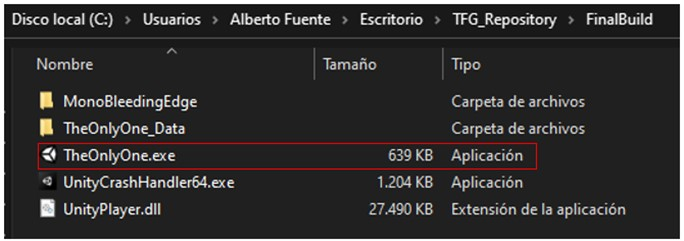
\includegraphics[scale=0.45]{img/GameExecution.jpg}
    \caption{Archivo de ejecución del videojuego}
    \label{fig:EjecucionJuego}
    \end{figure}
    
Después simplemente se tendrá que pulsar sobre el archivo ejecutable (.exe en Windows) para iniciar el videojuego (ver figura \ref{fig:EjecucionJuego}). El resto son archivos necesarios para que el videojuego pueda ejecutarse correctamente y almacenar los datos pertinentes.

\section{Manual del usuario}
En esta guía se enseñará al usuario de la aplicación a utilizarla debidamente paso por paso y qué podrá encontrar en cada rincón de la misma, así como los controles necesarios para poder jugar adecuadamente una vez se inicie la partida.

\subsection{Navegación por los menús}
Al iniciar el juego, tras mostrarse el logo de Unity, se presentará la pantalla de inicio de sesión.

Si se es la primera vez que se accede al juego, se deberá pulsar en el botón de ``Registrarse''. Este le llevará a la pantalla de registro, donde deberá introducir algunos datos para diferenciarse del resto de usuarios, como el nombre, el correo y una contraseña única (ver figura \ref{fig:PantallaRegistro}) (el correo no hace falta que sea real, simplemente tiene que contener el carácter ``@'').

\begin{figure}[h]
    \centering
    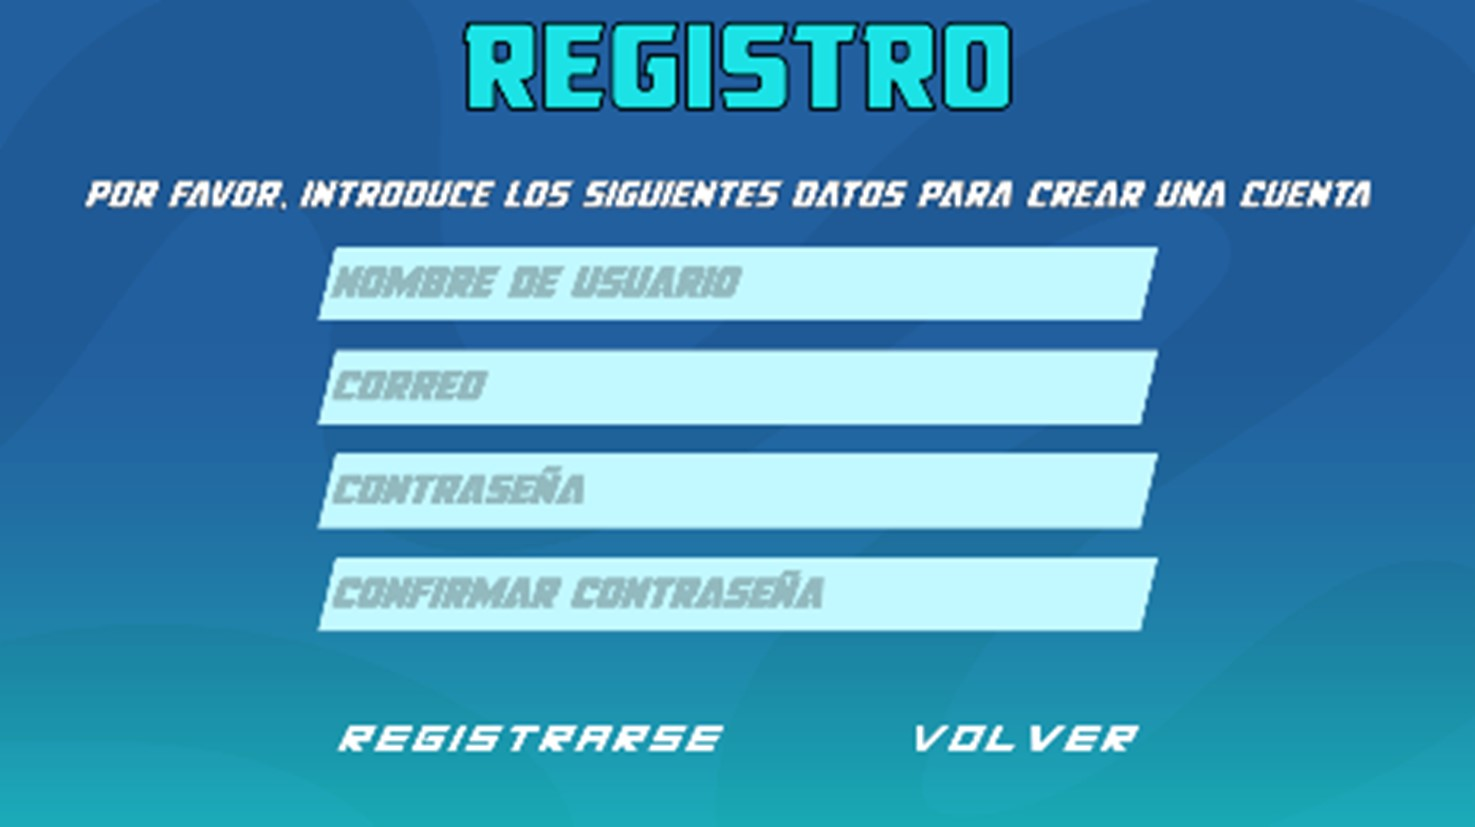
\includegraphics[scale=0.45]{img/SignUpScreen.jpg}
    \caption{Pantalla de registro}
    \label{fig:PantallaRegistro}
    \end{figure}
    
Una vez registrado, se volverá a la pantalla de inicio de sesión, donde podrá introducir el correo y la contraseña introducidos en el registro (ver figura \ref{fig:PantallaInicioSesión}).

\begin{figure}[h]
    \centering
    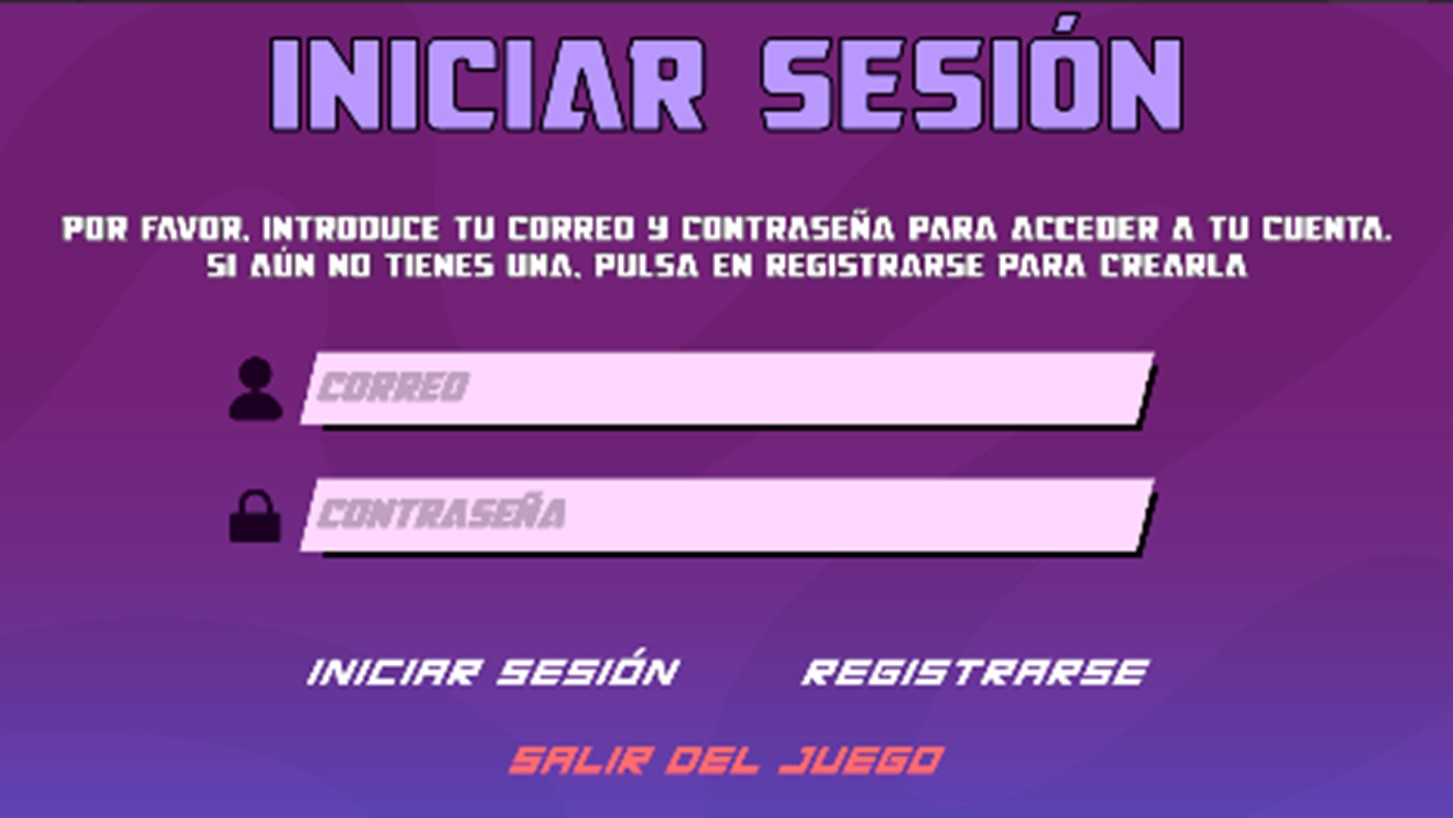
\includegraphics[scale=0.45]{img/LoginScreen.jpg}
    \caption{Pantalla de inicio de sesión}
    \label{fig:PantallaInicioSesión}
    \end{figure}
    
Si se introducen los datos correctamente, se cargará el menú principal del juego. En él, se pueden distinguir varias partes (ver figura \ref{fig:MenuPincipal}).

\begin{figure}[h]
    \centering
    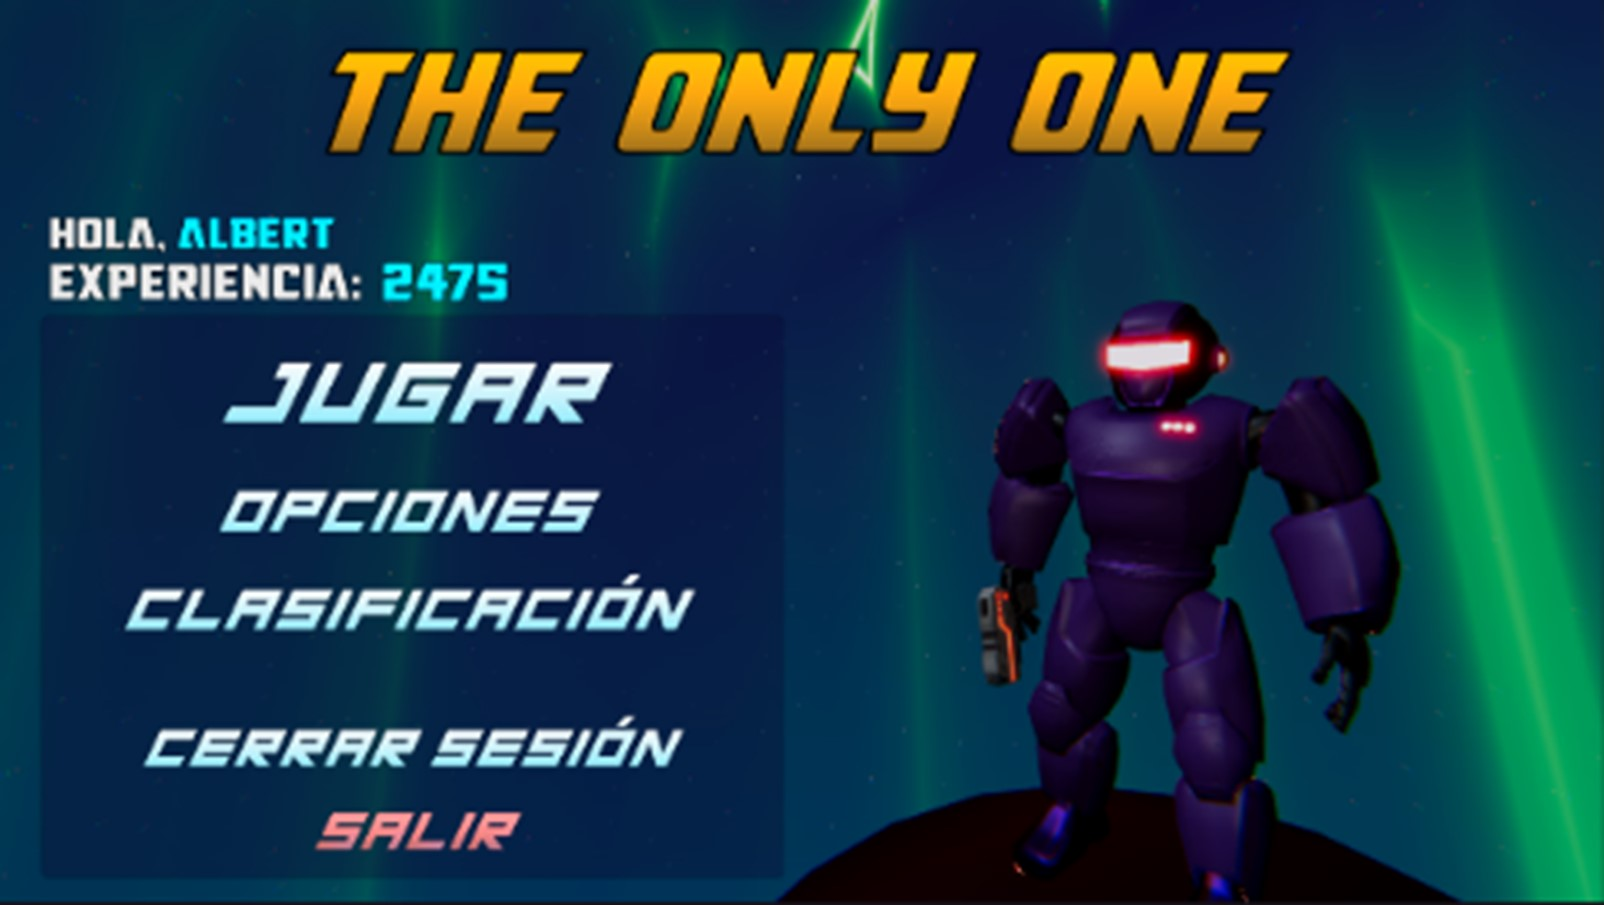
\includegraphics[scale=0.45]{img/MainMenu.jpg}
    \caption{Menú principal del videojuego}
    \label{fig:MenuPincipal}
    \end{figure}
    
En la parte superior se puede leer el nombre del juego: ``The Only One''. Justo debajo, se puede observar el nombre del usuario, que está resaltado en azul, así como la experiencia que tiene dicho usuario actualmente, también resaltada en azul.

Debajo de los datos del usuario se encuentra el propio menú, compuesto por diferentes botones, cada uno asociado a una acción diferente:

\begin{figure}[h]
    \centering
    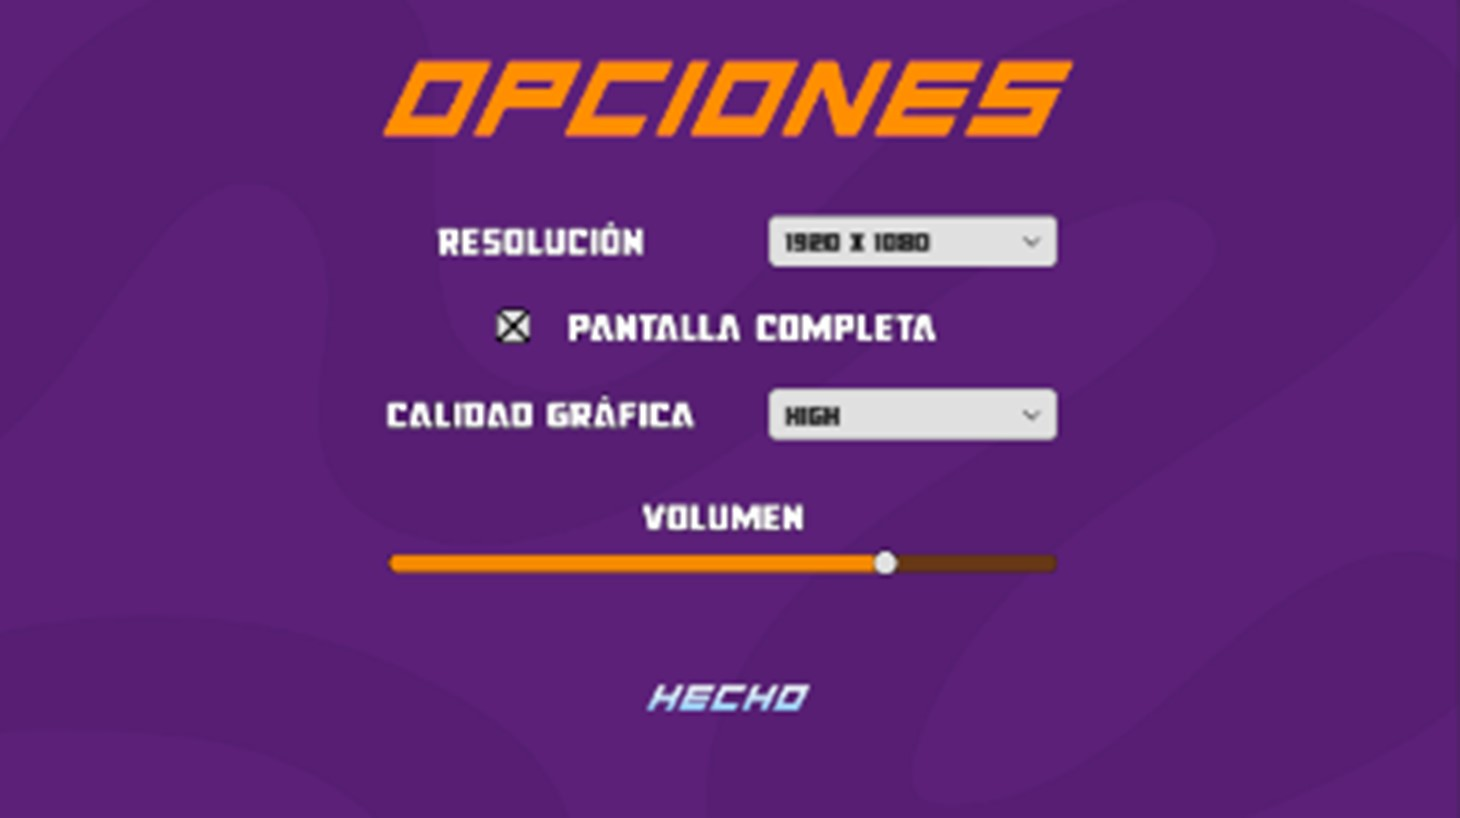
\includegraphics[scale=0.45]{img/OptionsScreen.jpg}
    \caption{Opciones técnicas disponibles}
    \label{fig:Opciones}
    \end{figure}
    
\begin{itemize}
    \item \textbf{Jugar}: Comienza una nueva partida.
    \item \textbf{Opciones}: Permite modificar algunos parámetros del juego (ver figura \ref{fig:Opciones}:
    \begin{itemize}
    \item \textbf{Resolución de la pantalla}: Se puede escoger entre varias resoluciones en función de lo que mejor se adapte a la pantalla en la que se muestra el videojuego.
    \item \textbf{Pantalla completa}: Permite elegir entre mostrar el juego en modo ventana u ocupando toda la pantalla.
    \item \textbf{Calidad gráfica}: Se pueden seleccionar tres clases de calidad para el aspecto visual del juego: \textit{Low} (baja), \textit{Medium} (media) o \textit{High} (alta). En función de la opción escogida, algunos elementos como las luces, sombras o los modelos tendrán más o menos calidad.
     \item \textbf{Volumen}: Permite ajustar el volumen general de los sonidos del juego.
    \end{itemize}
    \item \textbf{Clasificación}: Permite ver un ranking en forma de tabla de los jugadores con más puntos (experiencia) en el juego (ver figura \ref{fig:ClasificacionJugadores}). Uno de los objetivos de uso del juego es ganar experiencia para poder aparecer en las primeras posiciones de la tabla.
    
    \begin{figure}[h]
    \centering
    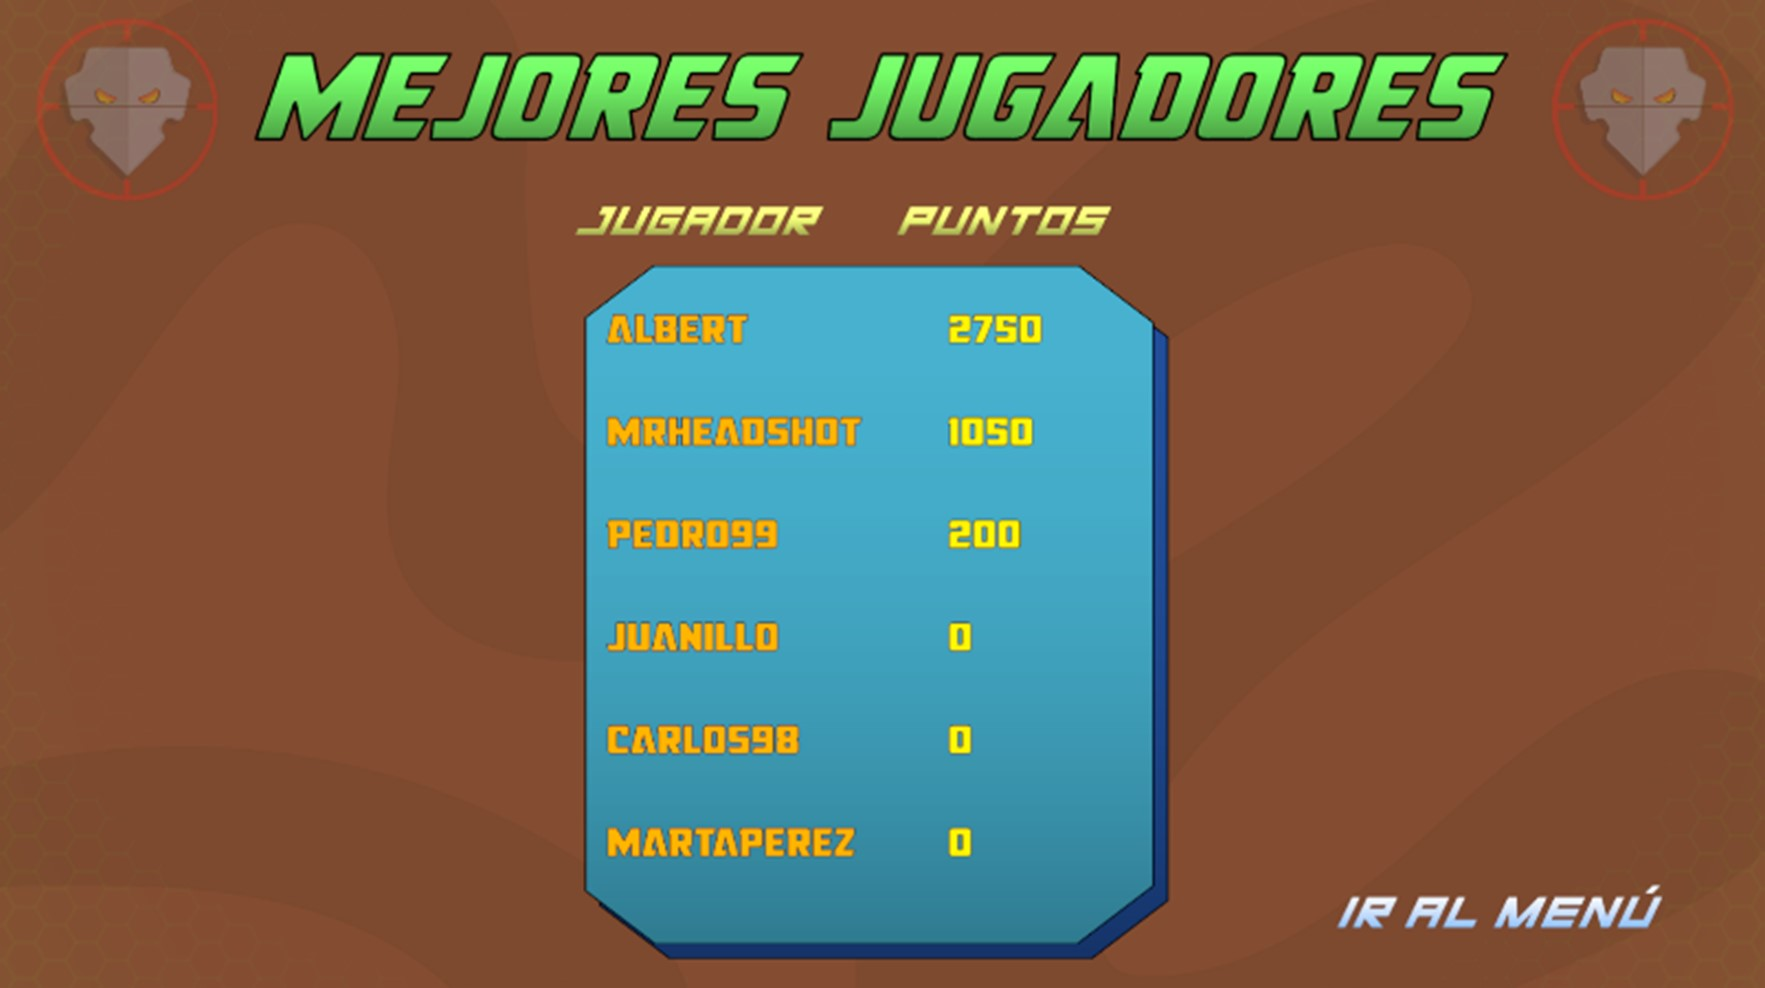
\includegraphics[scale=0.45]{img/RankingScreen.jpg}
    \caption{Tabla de clasificación de los mejores jugadores}
    \label{fig:ClasificacionJugadores}
    \end{figure}
    
    \item \textbf{Cerrar sesión}: Al pulsar esta opción, el usuario saldrá de su cuenta y volverá a mostrarse la pantalla de inicio de sesión. Cuando se termine una sesión de juego, es recomendable cerrar la sesión de la cuenta para que otros usuarios no puedan utilizarla sin autorización.
    \item \textbf{Salir}: Salir del juego.
\end{itemize}

\subsection{Desarrollo y controles del juego}
Al iniciar una partida, el jugador caerá desde el cielo a un mapa generado aleatoriamente, junto a otros 39 enemigos controlados por el ordenador. Todos ellos competirán para ser el último con vida, por lo que, para ganar la partida, el jugador deberá eliminar al resto de enemigos y ser el último en sobrevivir.

Para ello, el jugador debe ponerse en la piel del personaje al que controla, viendo el mundo desde su perspectiva, en primera persona.

Cuando cae del cielo, el jugador no tiene ningún equipamiento que le ayude a sobrevivir, por lo que lo primero que debe hacer es moverse para ir a buscar algo de armamento. Los controles básicos para manejar su movimiento son los siguientes (ver figura ):
\begin{itemize}
    \item \textbf{Mover el ratón}: El ratón controlará la cabeza del personaje, es decir, si se desea mirar a la izquierda, se debe mover el ratón a la izquierda, y si se desea mirar hacia abajo, se debe arrastrar el ratón hacia abajo, etc.
    \item \textbf{W/Flecha arriba}: Desplazarse hacia delante.
    \item \textbf{S/Flecha abajo}: Desplazarse hacia atrás.
    \item \textbf{A/Flecha izquierda}: Desplazarse hacia la izquierda.
    \item \textbf{D/Flecha derecha}: Desplazarse hacia la derecha.
    \item \textbf{Shift}: Correr. Es necesario tener pulsada al mismo tiempo alguna tecla de dirección (w,s,a,d)
    \item \textbf{Ctrl}: Agacharse, o, si se está sobre una pendiente pronunciada descendente, deslizarse.
    \item \textbf{Espacio}: Saltar
\end{itemize}
Con la combinación de estos controles básicos, el jugador puede explorar libremente el mapa que le rodea.

A medida que el jugador explore el mapa, se topará con diferentes elementos. Por ejemplo, hay \textbf{edificios y estructuras} que se pueden encontrar por todo el mapa. Para alcanzar las zonas más altas de estas estructuras, se pueden usar \textbf{plataformas de salto}, en las que, una vez subido, si el jugador salta, será impulsado con fuerza por el aire (ver figura \ref{fig:PlataformaSalto}).

\begin{figure}[h]
    \centering
    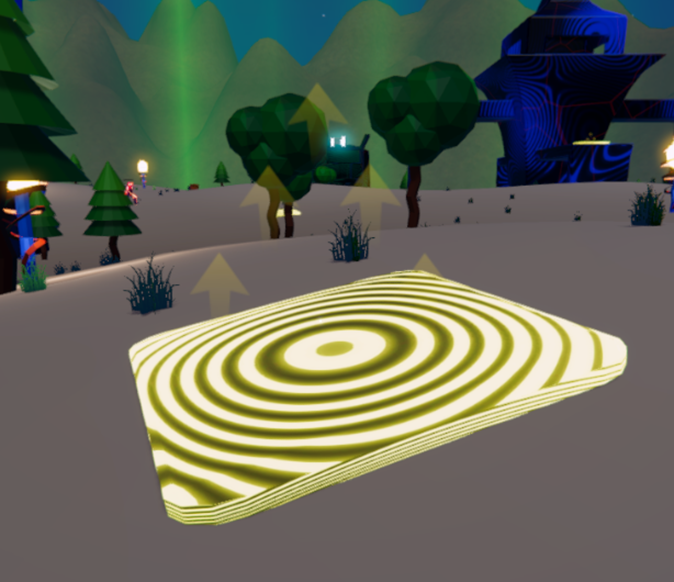
\includegraphics[scale=0.45]{img/bouncePlatform.png}
    \caption{Plataforma de salto}
    \label{fig:PlataformaSalto}
    \end{figure}

Algunas de las estructuras requieren de cierta habilidad para escalarlas. Una técnica para alcanzar zonas elevadas en las estructuras es corriendo por las paredes (\textbf{\textit{wallrun}}).\\
Para ello, el jugador debe tener una pared muy cerca, bien a su izquierda o a su derecha. Para subirse a ella, el usuario debe saltar al tiempo que presiona la tecla de dirección en la que se encuentre la pared. Una vez subido a la pared, tendrá un tiempo para moverse hacia avanzar o bien para impulsarse en dirección opuesta presionando la tecal de salto. Esta mecánica puede repetirse encadenando saltos para escalar paredes complicadas.

Es una mecánica algo complicada de dominar, que requiere práctica y coordinación, pero que una vez se sabe utilizar, es muy ventajosa para el jugador.

Se ha comentado el hecho de alcanzar lugares elevados o la parte superior de las estructuras porque es donde más cajas de suministros se pueden encontrar.
Las \textbf{cajas de suministros} (ver figura \ref{fig:CajaSuministros})son elementos que resultan de gran ayuda para el jugador, ya que contienen objetos aleatorios como packs de ayuda, armas o granadas, que benefician al jugador y le ayudan a ganar la partida más fácilmente.

\begin{figure}[h]
    \centering
    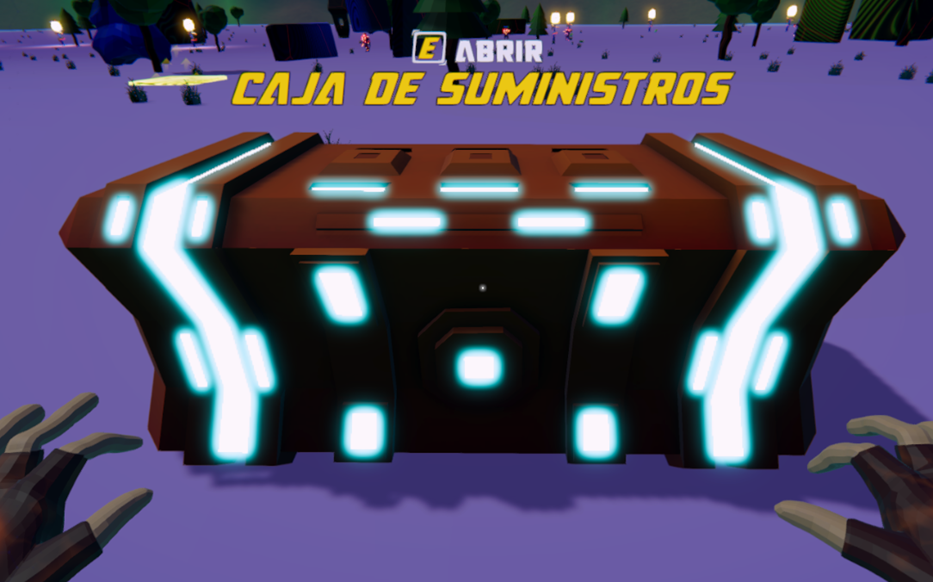
\includegraphics[scale=0.45]{img/Crate.png}
    \caption{Caja de suministros}
    \label{fig:CajaSuministros}
    \end{figure}

Cada tipo de objeto que el jugador puede encontrarse se describe a continuación, y dependiendo de la situación, convendrá utilizar unos u otros:
\begin{itemize}
    \item \textbf{Armas}. Las armas sirven para infligir daño a los enemigos y poder eliminarlos. Los tipos de armas disponibles son \textbf{pistola, escopeta, subfusil, rifle de asalto y francotirador} (ver figura \ref{fig:Armas}), y cada una con unas características diferentes, similares a las de las armas reales a las que imitan.\\
    
    \begin{figure}[h]
    \centering
    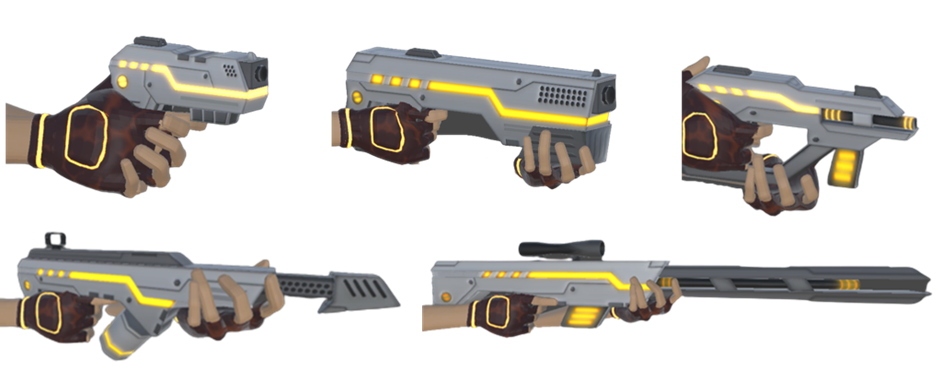
\includegraphics[scale=0.45]{img/WeaponSet.png}
    \caption{Armas disponibles en el juego}
    \label{fig:Armas}
    \end{figure}
    
    Por ejemplo, el francotirador es más conveniente cuando se quiere alcanzar a un enemigo que se encuentre a una gran distancia, mientras que la escopeta solo inflige daño en distancias cortas.
    \item \textbf{Granadas}. Son objetos arrojables que, tras unos segundos, explotan y harán diferentes cosas depediendo de su tipo. Hay dos tipos de granadas en el juego:
    \begin{itemize}
        \item \textbf {Granada explosiva}: Hace un gran daño a los enemigos que se encuentren en su radio de explosión.
        \item \textbf {Granada de hielo}: Congela durante unos segundos a los enemigos que se encuentren en su radio de acción. Durante ese tiempo, permanecerán inmóviles sin poder atacar al jugador.
    \end{itemize}
    \item \textbf{Packs de ayuda}. Son objetos que otorgan al jugador distintas cosas en función de su tipo:
    \begin{itemize}
        \item \textbf {Pack de salud}: Hace que el jugador recupere cierta cantidad de vida.
        \item \textbf {Pack de armadura}: Hace que el jugador recupere cierta cantidad de armadura.
        \item \textbf{Pack de munición}. Añade munición de reserva a las armas equipadas.
    \end{itemize}
\end{itemize}
Un elemento a tener en cuenta es el \textbf{Inventario}, una especie de mochila donde el jugador puede llevar consigo tanto armas como granadas, y utilizar cada una según sea más conveniente (ver figura \ref{fig:Inventario}).

\begin{figure}[h]
    \centering
    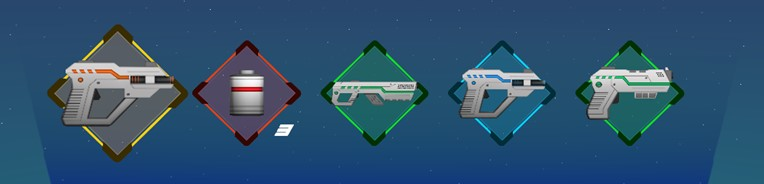
\includegraphics[scale=0.45]{img/InventoryInterface.jpg}
    \caption{Inventario del jugador}
    \label{fig:Inventario}
    \end{figure}

Respecto a las armas y a los packs de ayuda, es importante saber que pueden tener distintas rarezas (común(azul), rara(verde), épica(morado) y legendaria(amarillo) (ver figura \ref{fig:Rarezas}). Cada rareza definirá las estadísticas del objeto asociado. Por ejemplo, un pack de salud común recupera 25 puntos de vida al jugador, mientras que uno épico recupera 75.

\begin{figure}[h]
    \centering
    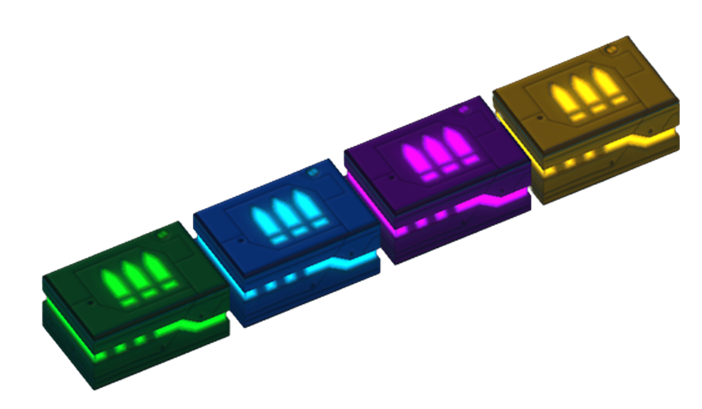
\includegraphics[scale=0.45]{img/Packs.png}
    \caption{Rarezas del juego}
    \label{fig:Rarezas}
    \end{figure}

Obviamente, será más complicado encontrar los objetos de mayor rareza. Concretamente, la probabilidad de que apareza cada tipo de objeto es 50\% para los comunes, 30\% para los raros, 15\% para los épicos y 5\% para los legendarios.

Por lo tanto, el jugador siempre deberá priorizar equipar o conusmir objetos de mayor rareza.

Para poder utilizar adecuadamente los objetos descritos, se deben conocer algunos controles de acción además de los de movimiento:
\begin{itemize}
    \item \textbf{E}: Interactuar. Es una tecla que hará varias cosas en función del objeto con el que se interactúe (ver figura \ref{fig:Interactuar}):
    \begin{itemize}
        \item Abrir una caja de suministros.
        \item Equipar arma o granada.
        \item Consumir pack de salud, armadura o munición.
        \end{itemize}
        
        \begin{figure}[h]
    \centering
    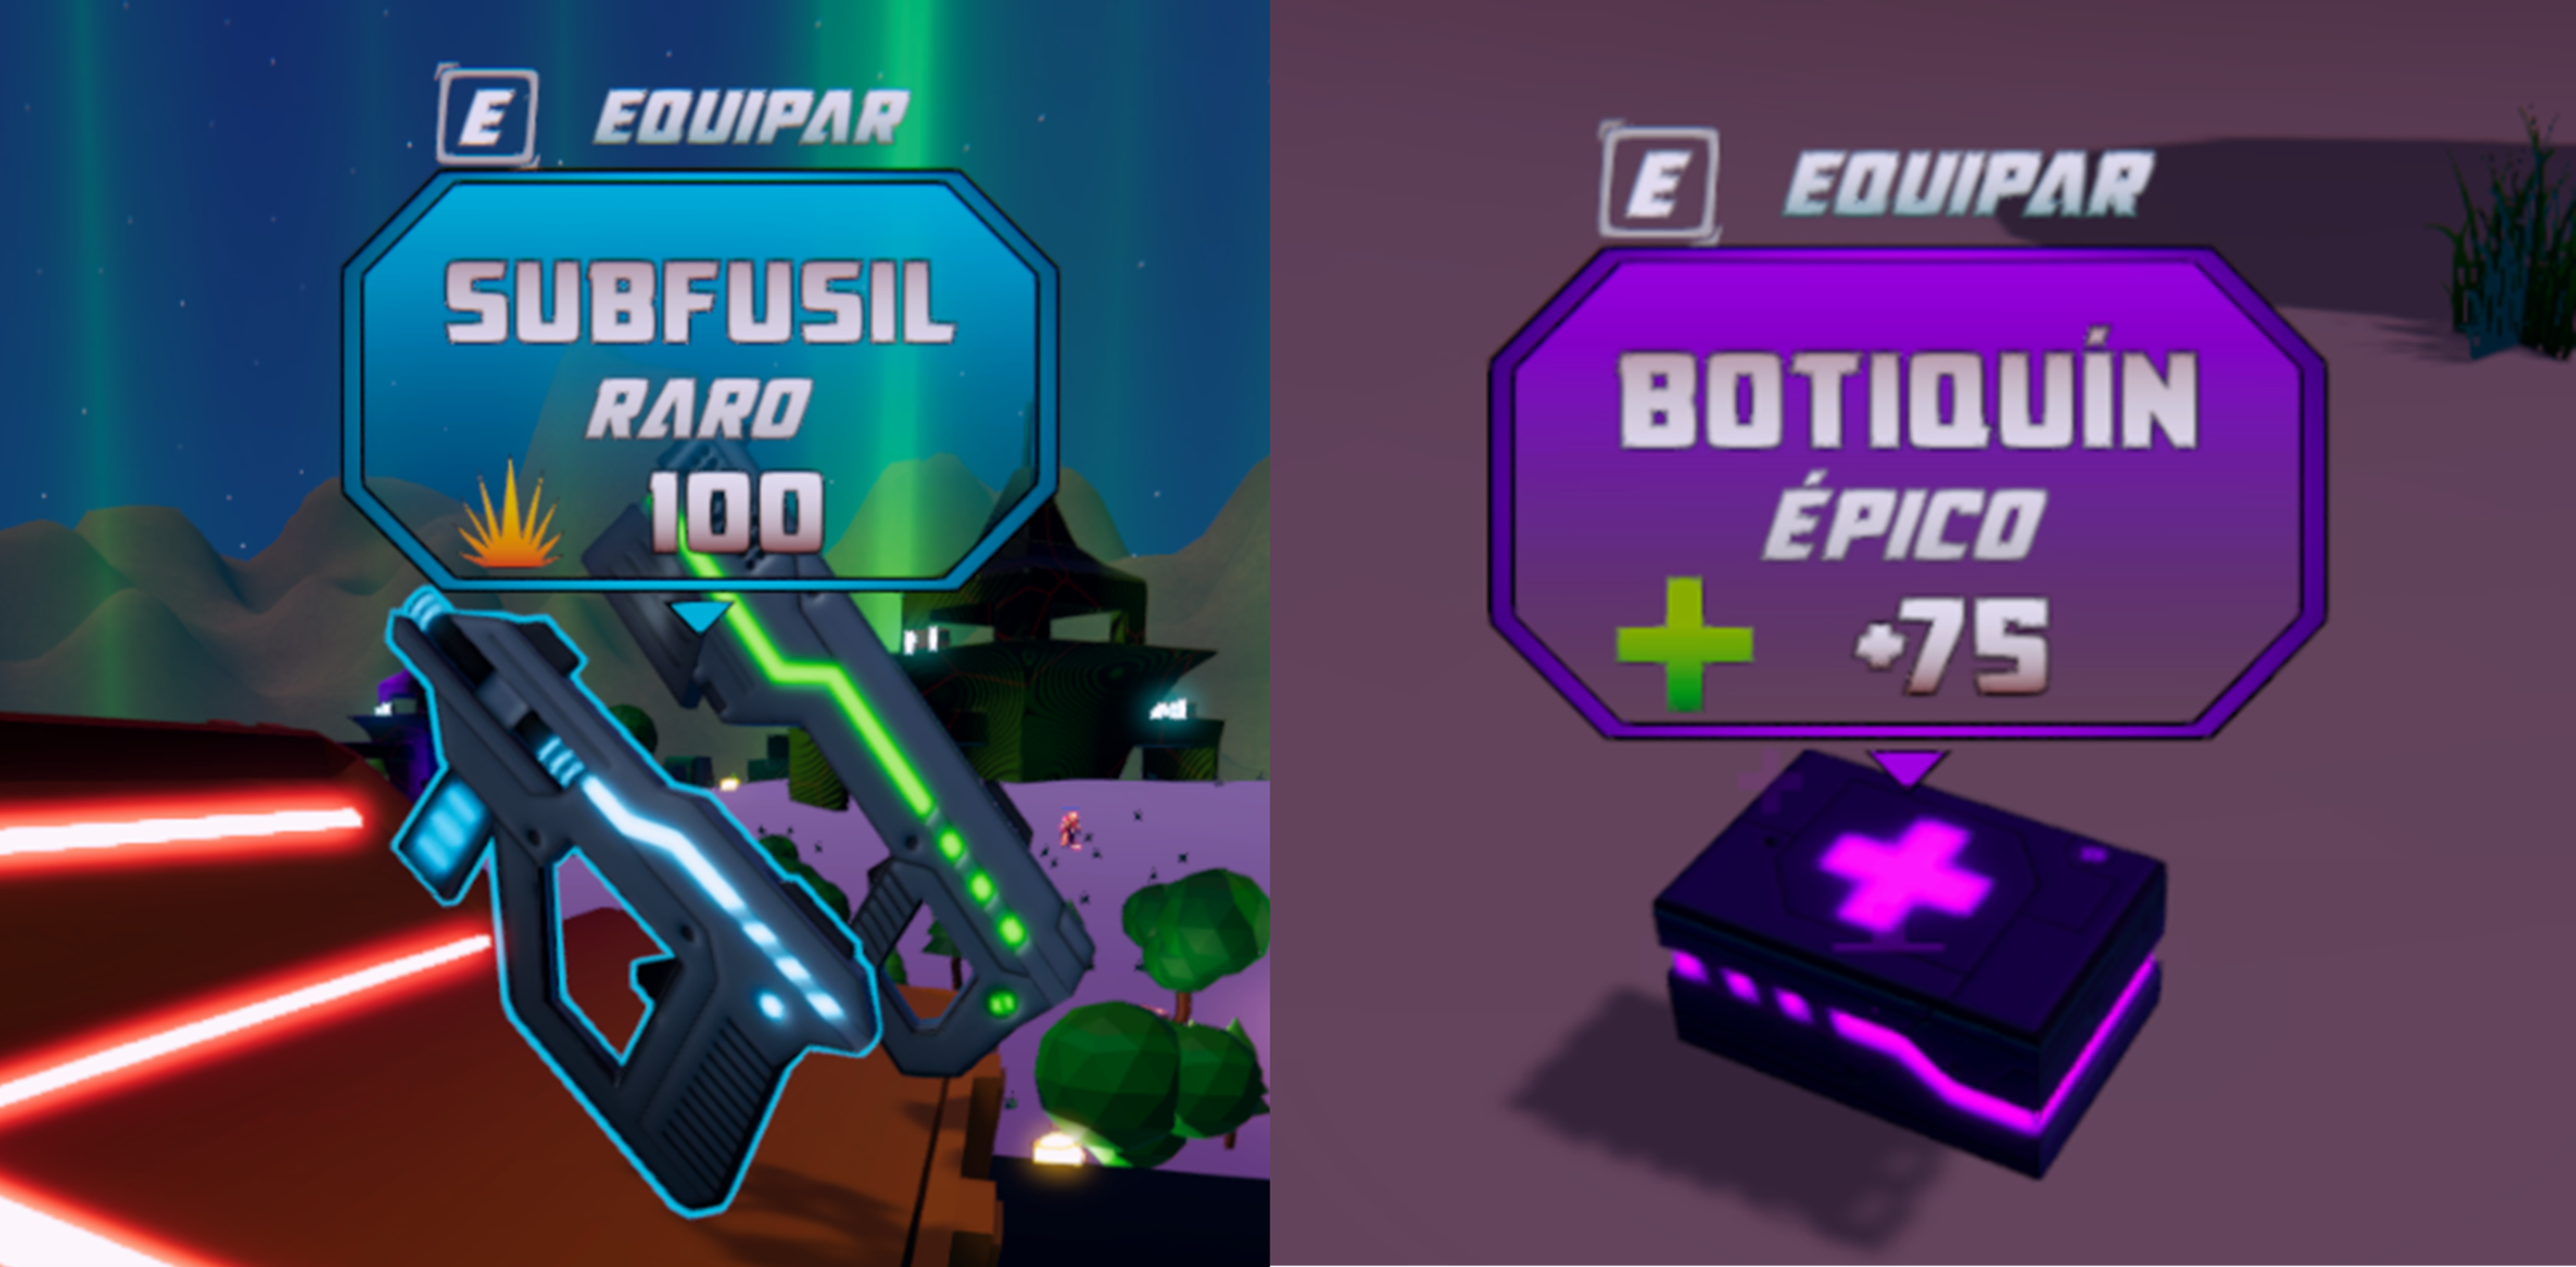
\includegraphics[scale=0.45]{img/LabelExamples.png}
    \caption{Interactuar con objetos}
    \label{fig:Interactuar}
    \end{figure}
    
    \item \textbf{Q}: Soltar objeto. Tira el objeto activo al suelo, vaciando su compartimento del inventario.
    \item \textbf{Rueda del ratón}: Cambiar de objeto activo. Al hacer \textit{scroll} con la rueda del ratón, el jugador podrá seleccionar cualquier objeto que tenga en el inventario en ese momento.
    \item \textbf{click izquierdo}: Utilizar objeto. En el caso de las granadas, servirá para lanzarlas, y en las armas, hará que se disparen. Además, en las armas automáticas (subfusil y rifle de asalto), se puede mantener pulsado para que se disparen varios proyectiles de forma continuada.
    \item \textbf{click derecho}: Apuntar. Si se quiere ganar precisión utilizando las armas, se puede apuntar para hacer que el arma se posicione en el centro de la pantalla, se haga zoom en la imagen y se disminuya el retroceso del arma. Esto es muy útil por ejemplo en grandes distancias donde es difícil concentrar la mirilla en un punto lejano.
    \item \textbf{R}: Recargar. A medida que se utilicen las armas, se irán agotando las balas de su cargador. En cualquier momento, y siempre que haya balas disponibles, se puede llenar el cargador de nuevo para poder seguir disparando.
\end{itemize}
El jugador debe mantenerse con vida en todo momento para poder ganar la partida, y por ello debe evitar que los enemigos le disparen, bien matándolos a tiempo, alejándose de ellos o cubriéndose con algún elemento del mapa.

Además, debe mantenerse siempre dentro de la zona segura del mapa, delimitada en forma circular por una nube tóxica, que irá reduciendo progresivamente el tamaño de la zona segura (ver figura \ref{fig:NubeToxica}).\\
En caso de encontrarse fuera de este área, el jugador se intoxicará e irá recibiendo daño constantemente hasta que vuelva a la zona segura.

\begin{figure}[h]
    \centering
    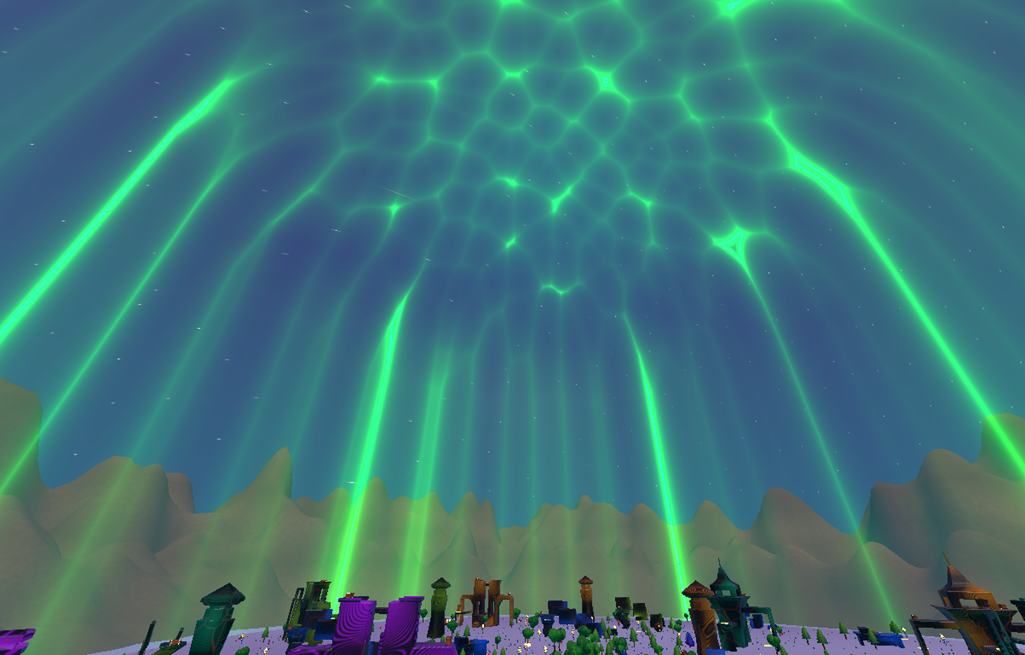
\includegraphics[scale=0.45]{img/ToxicCloud.png}
    \caption{Nube tóxica del juego}
    \label{fig:NubeToxica}
    \end{figure}
    
La vida del jugador está delimitada por dos componentes: su \textbf{armadura} y su \textbf{salud}, representadas en el HUD con dos barras de color azul y verde, respectivamente (ver figura \ref{fig:BarrasVida}).\\
Si el jugador tiene armadura restante, cuando reciba daño, se irá rompiendo esta armadura hasta que se rompa por completo, y entonces empezará a disminuir su salud. Si no, bajará su salud directamente.
Si la salud del jugador llega a cero, pierde la partida, y por ello es importante que evite al máximo ser disparado por los enemigos, y deberá consumir packs de vida y armadura para rellenarlas.
\begin{figure}[h]
    \centering
    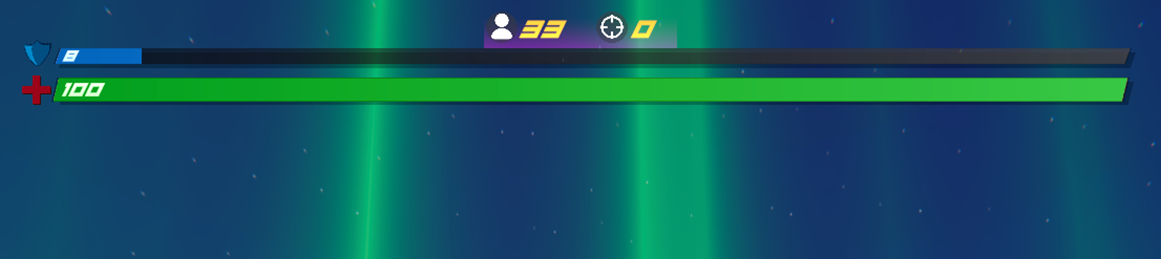
\includegraphics[scale=0.37]{img/HealthBars.png}
    \caption{Barras de vida del jugador}
    \label{fig:BarrasVida}
    \end{figure}













